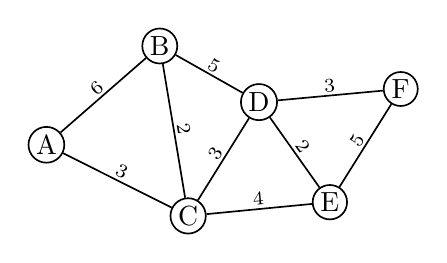
\begin{tikzpicture}[scale=1.8,node distance=1.5cm,semithick,inner sep=1pt,bend angle=45,sloped,anchor=south]
%\draw[help lines] (-3,-3) grid (3,0);
\node[circle,draw] (A)  at(0,0)    {A};
\node[circle,draw] (B)  at(0.8,0.7) {B};
\node[circle,draw] (C)  at(1,-0.5) {C};
\node[circle,draw] (D)  at(1.5,0.3) {D};
\node[circle,draw] (E)  at(2,-0.4) {E};
\node[circle,draw] (F)  at(2.5,0.4) {F}; 

\path
(A)  edge node{\scriptsize $6$} (B)
     edge node{\scriptsize $3$} (C)
(B)  edge node{\scriptsize $2$} (C)
     edge node{\scriptsize $5$} (D)
(C)  edge node{\scriptsize $3$} (D)
     edge node{\scriptsize $4$} (E)
(D)  edge node{\scriptsize $2$} (E)
     edge node{\scriptsize $3$} (F)
(E)  edge node{\scriptsize $5$} (F);  
 

\end{tikzpicture}
